\section{Architecture}

\begin{figure*}[!t]
\centering
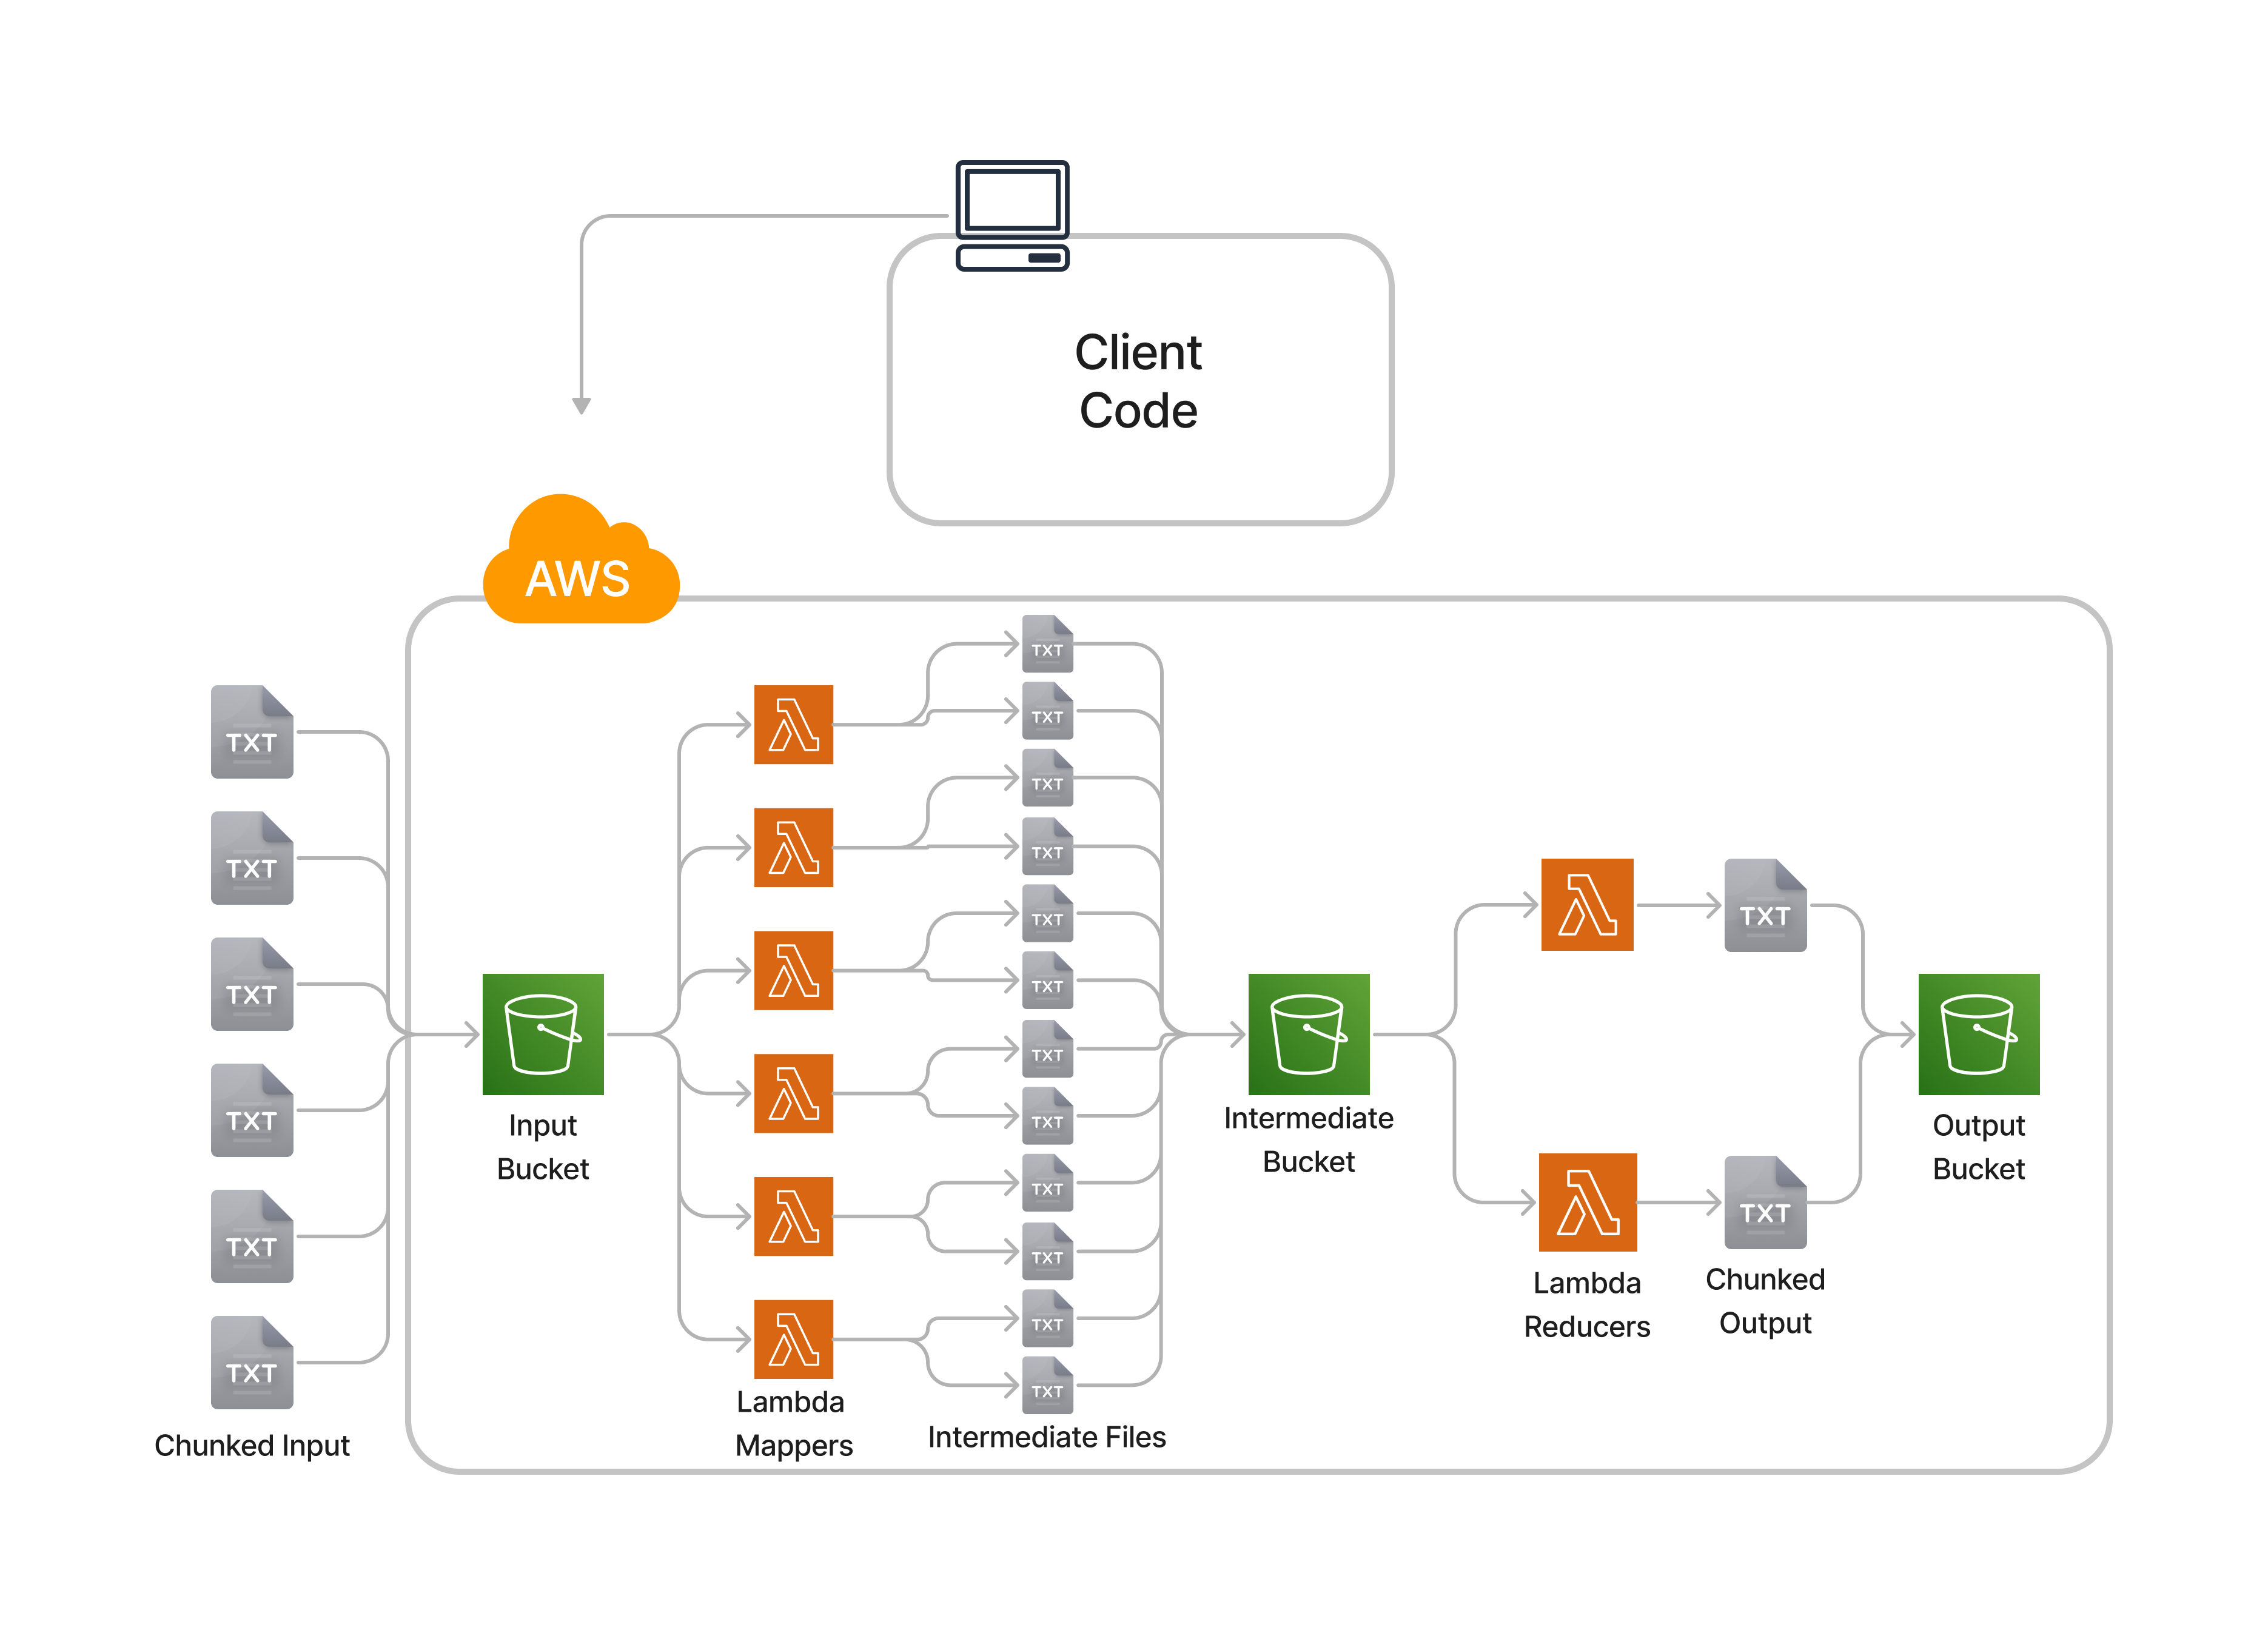
\includegraphics[width=\textwidth]{project_latex_template/images/arch.png}
\captionof{Figure 1.}{\small{ Architecture of the Serverless MapReduce runtime}}
\label{fig:arch}
\end{figure*}

In this section, we describe the architecture of our serverless MapReduce runtime and its functioning. The entire application consists of various parts like the client-side code, AWS S3 buckets, AWS Lambda functions and their associated code, and ancillary scripts for evaluation and testing. All code is written in Python. A detailed overview of the architecture is shown in Figure 1, with six mappers and two reducers.

\subsection{Components}

In order to make a Serverful MapReduce implementation work, two main components are needed: machines (or "nodes") that run the map or reduce jobs and an underlying distributed file system for sharing data. Google's implementation of MapReduce used the Google File System~\cite{ghemawat2003google} as the distributed file system. In our implementation, we used AWS S3- Amazon's highly scalable object store- as our distributed file system. Instead of long-running servers that run map or reduce tasks, our Serverless implementation will use short-lived AWS Lambda functions. Just like any other MapReduce implementation, the user defines \emph{Map(Key, Value)} and \emph{Reduce(Key, Value List)} functions based on their specific task.

The Serverless MapReduce implementation is supported by the following main components:

\begin{itemize}
    \item \emph{Input Bucket}: The input bucket stores the input corpus chunked into many files. The number of mappers invoked (\emph{m}) is equal to the number of chunks the input is divided into. Since Lambda is built for concurrent executions, this allows us to scale our workloads in a massively parallel manner by chunking the input as much as possible, beyond what may be possible for a Serverful implementation.
    
    \item \emph{Lambda Mappers}: When a Lambda Mapper is invoked, it is passed the input file and the number of reducers (\emph{n}) defined by the client. The mapper calls the user-defined \emph{Map(Key, Value)} on the file contents to obtain the intermediate key-value pairs. The mapper bins the intermediate key-value pairs based on the equation:
    \[bucket = hash(key) \pmod{n}\]
    Each of the \emph{n} intermediate files is encoded as JSON and stored in the intermediate bucket.
    
    \item \emph{Intermediate Bucket}: Each Mapper Lambda emits \emph{n} intermediate files that contain JSON-encoded key-value pairs and are stored in the intermediate S3 bucket. The total number of intermediate files for a given MapReduce job is $m\times{n}$. The files follow the naming convention:
    \[\emph{ReducerID\_InputChunkUID.json}\]
    Here, $ReducerID \in [0,n-1]$ and $InputChunkUID$ is a unique identifier associated with each input chunk. This naming convention is used by the runtime to figure out what reducers can be run and the files that need to be assigned to each reducer.
    
    \item \emph{Lambda Reducers}: When a Reducer Lambda is invoked, it is passed a list of all the intermediate files it needs to read and the \emph{ReducerID}. After reading all the relevant JSON data, the reducer transforms the key-value pairs into (key, value list) format. That is, for each unique key, we have a list of all the values associated with that key. The user-defined \emph{Reduce(Key, Value list)} function is called for each unique key to obtain the final output, which is encoded as JSON.
    
    \item \emph{Output Bucket}: Each of the \emph{n} reducers writes one file to the output bucket. To obtain the aggregate output of the MapReduce job, all the output chunks may have to be combined. If the output is in key-value pair form, it may be used as the input for another MapReduce job.
    
    \item \emph{Serverless MapReduce Client}: The Serverless MapReduce Client is the application the user interacts with to submit their MapReduce job. The main parameters the user has to specify are the S3 input bucket that contains the chunked input files and the number of reducers desired (\emph{n}).

    \item \emph{Miscellaneous Components}: Other parts of the system include AWS IAM roles and permission policies that allow communication between the various AWS services and ancillary components for combining output bucket data and comparing it against known values to validate the system.
\end{itemize}

Each Lambda was allocated a memory of 256 MB, 512 MB storage, and a timeout of 2 minutes.

\subsection{Workflow}

A typical run of a Serverless MapReduce job looks as follows:

\begin{enumerate}
    \item The user specifies their input bucket and the number of reducers (\emph{n}) and runs the MapReduce client.
    \item The MapReduce client invokes a Mapper Lambda for each input chunk. This can potentially be thousands of mappers.
    \item The Mapper Lambda stores its intermediate files (containing intermediate key-value pairs) in the intermediate bucket.
    \item Depending on what intermediate files have been written to the intermediate bucket, the MapReduce client figures out if any Reducer Lambdas are ready to run and invokes them until all \emph{n} reducers have been invoked.
    \item Once all the reducers are done, the chunked output is stored in the output S3 bucket. At this point, the output may be aggregated or passed on to another MapReduce job.
\end{enumerate}

\section{Testing}

To evaluate the correctness of our MapReduce implementation and benchmark its performance, we decided to use the classic word count MapReduce task. We used books from the Project Gutenberg library to create input data sets of various sizes for our testing. The user-defined map and reduce functions for this task are presented below. This is the only thing the user has to specify in addition to the input files and number of reducers.

\begin{algorithm}
\caption{Map Function For Word Count}
\begin{algorithmic}[1]
\Function{UserMapFunction}{$k, v$}
    \State $words \gets [filtered~words~from~v]$
    \State $kv\_list \gets []$
    \For{$word$ \textbf{in} $words$}
        \State $kv\_list$.append(($word$.lower(), 1))
    \EndFor
    \State \Return $kv\_list$
\EndFunction
\end{algorithmic}
\end{algorithm}

\begin{algorithm}
\caption{Reduce Function For Word Count}
\begin{algorithmic}[2]
\Function{UserReduceFunction}{$k, \text{val\_list[]}$}
    \State \Return $\text{len}(\text{val\_list})$
\EndFunction
\end{algorithmic}
\end{algorithm}

\subsection{Methodology}

Using different books from the Project Gutenberg repository, we created test cases of increasing sizes. The number of Mapper Lambdas invoked is equal to the number of input files or chunks, and the number of Reducer Lambdas invoked is specified by the user. We created three total test cases: small, medium, and large. These scale from tens of Lambdas to about a thousand concurrently executing Lambda functions.

The different testing scenarios and their average completion times are presented in Table I. The current configurations allow 1,000 concurrent Lambda invocations, so some throttling was observed in the largest test case.

Each test scenario was run five times to obtain the average completion time across all runs. The number of reducers used was scaled appropriately based on how many input chunks each test scenario had. Making the number of reducers too small would result in Lambda invocations timing out as each reducer was overloaded with a lot more work, causing it to use up all its working memory and not finish before the timeout.

\subsection{Results}
